
\documentclass[border=0pt]{standalone}
\usepackage{tikz}
\usetikzlibrary{shapes.geometric, positioning, calc}
\usetikzlibrary{decorations.pathreplacing}
\usepackage{amsmath}

\begin{document}

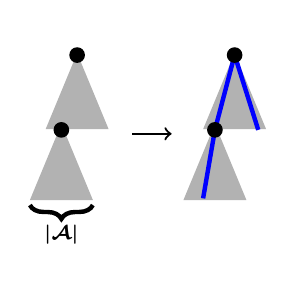
\begin{tikzpicture}[level distance=1.5cm, sibling distance=2cm, 
    every node/.style={font=\scriptsize}]

    % Left tree (SOTA methods considering all actions)
    \node[isosceles triangle, rotate=90, fill=gray!60, minimum size=0.8cm, behind path] (B1) at (0, -0.7){};
 
    \node[behind path, isosceles triangle, rotate=90, fill=gray!60, minimum size=0.8cm] (C1) at (-0.2, -1.6){};
    % Label for action space |A|
    \draw [ultra thick, decorate,decoration={brace,amplitude=5pt,mirror,raise=4ex}]
  (-0.6,-1.3) -- (0.2,-1.3) node[midway,yshift=-2.8em]{$\boldsymbol{|\mathcal{A}|}$};
    % \node[below left= 0.1cm of C1] {$|\mathcal{A}|$};
    \node[circle, fill=black, inner sep=2pt, label=above:{}] (A1) at(0, 0){};
    \node[circle, fill=black, inner sep=2pt, label=above:{}] (A2) at (-0.2, -0.95){};

    
    \node[isosceles triangle, rotate=90, fill=gray!60, minimum size=0.8cm] (B1) at (2, -0.7){};
    
    % add a right arrow
    \draw[->, thick] (0.7, -1) -- (1.2, -1);
    
    \node[isosceles triangle, rotate=90, fill=gray!60, minimum size=0.8cm] (B2) at (1.75, -1.6){};
    \draw[-, blue, ultra thick] (2, 0) -- (1.75, -0.95);
    \draw[-, blue, ultra thick] (2, 0) -- (2.3, -0.95);

    \draw[-, blue, ultra thick] (1.75, -0.95) -- (1.6, -1.82);
    % \draw[-, blue, ultra thick] (1.75, -1.2) -- (1.8, -2.4);
    
    \node[circle, fill=black, inner sep=2pt] (O1) at (2, 0){};
    \node[circle, fill=black, inner sep=2pt] (O2) at (1.75, -0.95){};
    

\end{tikzpicture}

\end{document}